\documentclass[a4paper,leqno,12pt]{amsart}
%
\usepackage{amsmath,amsthm}
\usepackage{graphicx}
\usepackage[margin=0.7in]{geometry}

\usepackage{enumitem}

\usepackage{multirow}
\usepackage{tikz}
\usepackage{wrapfig}
\usepackage[autostyle=true]{csquotes}

\usepackage{fancyhdr}
\pagestyle{fancy}
\fancyhf{} % clear all header/footer fields
\fancyfoot[C]{\bf ************************************} % 

\newlist{Case}{enumerate}{1}
\setlist[Case]{label=\bf{Case ~\arabic*:}}
%
\begin{document}
\hspace*{1.9cm}% <-- adjust this value to push everything right
\begin{tabular}{@{}p{0.7\textwidth}p{0.3\textwidth}@{}}
 {\raggedright
   \begin{center} 
   \textbf{AZIM PREMJI UNIVERSITY, BHOPAL}\\
   First Semester 2026--2027 \\
   Tutorial Sheet--2
   \end{center}
  } %&
  %{\raggedleft
   %
\includegraphics[width=3cm]{Azim_Premji_University_logo.png} % replace logo.png with your file name
 % }
\end{tabular}

\noindent Course No. MTH-113 \hfill  Course title: Introduction to Quantitative Thinking
%\vspace{.3cm}
\hrule 
\vspace{.1cm}


\begin{enumerate}
\setlength\itemsep{1em}
\item Write the fraction representing the shaded reason of each color in the below pictures\\

(a)
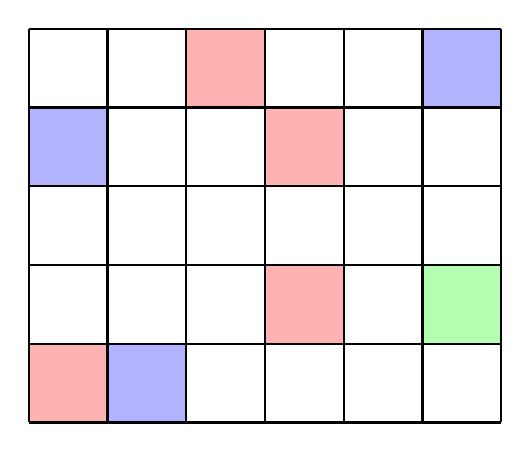
\begin{tikzpicture}
  \fill[blue!30] (1,1) rectangle (2,2); % cell at (1,1)
  \fill[blue!30] (0,4) rectangle (1,5);
  \fill[blue!30] (5,5) rectangle (6,6);
  \fill[red!30] (3,4) rectangle (4,5); % cell at (3,4)
  \fill[red!30] (2,5) rectangle (3,6);
  \fill[red!30] (3,2) rectangle (4,3);
   \fill[red!30] (0,1) rectangle (1,2);
  \fill[green!30] (5,2) rectangle (6,3); % cell at (5,2)

  \draw[thick] (0,1) grid (6,6);

  % Shade some cells
\end{tikzpicture}
\quad
(b)

\begin{tikzpicture}
 \fill[red!30] (0,0) -- (-0.5,1) -- (0.5, 1);
 \fill[red!30] (1,2) -- (0.5,1) -- (0,2);

 \draw[thick] (-1,2) -- (1,2);
 \draw[thick] (-1,2) -- (0,0);
 \draw[thick] (1,2) -- (0,0);
 
 \draw[thick] (0,2) -- (-0.5, 1);
 \draw[thick] (0,2) -- (0.5, 1);
 \draw[thick] (-0.5, 1) -- (0.5, 1);
 
\end{tikzpicture}
\quad
(c)
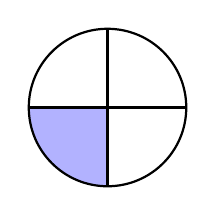
\begin{tikzpicture}
 \fill[blue!30] (0,0) -- (0,-1) arc (270:180:1) circle;

 \draw[thick] (0,0) circle [radius=1];
 \draw[thick] (0,1) -- (0,-1);
 \draw[thick] (-1,0) -- (1,0);
 
\end{tikzpicture}

\item Shade the part according to the given fraction. \\

(a)  $\frac{1}{6}$
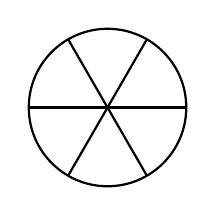
\begin{tikzpicture}
 \draw[thick] (0,0) circle [radius=1];
 
 \foreach \angle in {0, 60, 120, 180, 240, 300}
 	\draw[thick] (0,0) -- (\angle:1);
\end{tikzpicture}
\quad
(b) $\frac{1}{4}$
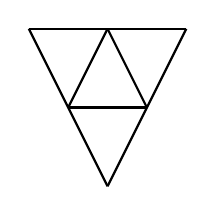
\begin{tikzpicture}
 \draw[thick] (-1,2) -- (1,2);
 \draw[thick] (-1,2) -- (0,0);
 \draw[thick] (1,2) -- (0,0);
 
 \draw[thick] (0,2) -- (-0.5, 1);
 \draw[thick] (0,2) -- (0.5, 1);
 \draw[thick] (-0.5, 1) -- (0.5, 1);
\end{tikzpicture}
\quad
(c) $\frac{4}{9}$
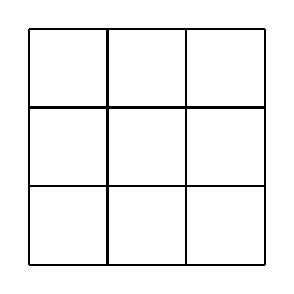
\begin{tikzpicture}
 \draw[thick] (0,0) grid (3,3);
\end{tikzpicture}

\item Identify the errors if any \\
(a) 
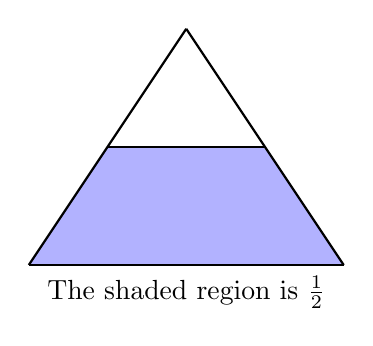
\begin{tikzpicture}
 \fill[blue!30] (-1,1.5) -- (1,1.5) --  (2,0) -- (-2,0) --cycle;
 \draw[thick] (0,3) -- (-2,0);
 \draw[thick] (0,3) -- (2,0);
 \draw[thick] (-2,0) -- (2,0);
 
 \draw[thick] (-1,1.5) -- (1,1.5);
 \node[below] at (current bounding box.south) {The shaded region is $\frac{1}{2}$};
\end{tikzpicture}
\quad
(b)
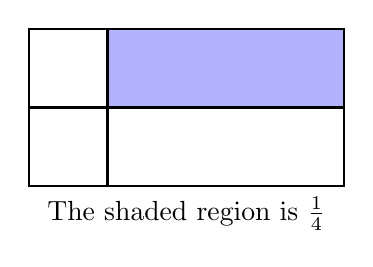
\begin{tikzpicture}
 \fill[blue!30] (1,1) -- (1,2) -- (4,2) -- (4,1) -- cycle;

 \draw[thick] (0,0) rectangle (4,2);
 \draw[thick] (1,0) -- (1,2);
 \draw[thick] (0,1) -- (4,1);
  \node[below] at (current bounding box.south) {The shaded region is $\frac{1}{4}$};
\end{tikzpicture}

\item 
\begin{enumerate}
 \item What fraction of a day is 8 hours?
 \item What fraction of an hour is 40 minutes?
\end{enumerate}

\item Arya, Abhimanyu, and Vivek shared lunch. Arya has brought two sandwiches,
one made of vegetable and one of jam. The other two boys forgot to bring their
lunch. Arya agreed to share his sandwiches so that each person will have an
equal share of each sandwich.
\begin{enumerate}
 \item How can Arya divide his sandwiches so that each person has an equal share?
 \item What part of a sandwich will each boy receive?
\end{enumerate}

\item Kanchan dyes dresses. She had to dye 30 dresses. She has so far finished 20
dresses. What fraction of dresses has she finished?

\item Write the natural numbers from 2 to 12. What fraction of them are prime numbers?

\item A fraction is given.\\
How will you decide, by just looking at it, whether, the fraction is
\begin{enumerate}
 \item less than 1?
 \item equal to 1?
\end{enumerate}

\item Fill up using one of these:  \enquote{$>$},  \enquote{$<$} or \enquote{=} \\

(a) $\frac{1}{2} \ \square \ 1 \quad$ (b) $\frac{3}{5} \ \square \ 1 \quad$ (c) $1 \ \square \ \frac{7}{8} \quad$ (d) $\frac{4}{4} \ \square \ 1 \quad$
 
\item Draw number lines and locate the points on them:\\

(a) $\frac{1}{2}, \frac{1}{4}, \frac{3}{4}, \frac{4}{4}$ \quad (b) $\frac{1}{8}, \frac{2}{8}, \frac{3}{8}, \frac{7}{8}$ \quad (c) $\frac{2}{5}, \frac{3}{5}, \frac{8}{5}, \frac{4}{5}$

\item Express the following as mixed fractions:\\

(a) $\frac{20}{3}$ \quad (b) $\frac{11}{5}$ \quad (c) $\frac{17}{7}$ \quad (d) $\frac{28}{5}$ \quad (e) $\frac{19}{6}$ \quad (f) $\frac{35}{9}$

\item Express the following as improper fractions:\\

(a) $7\frac{3}{4}$ \quad (b) $5\frac{6}{7}$ \quad (c) $2\frac{5}{6}$ \quad (d) $10\frac{3}{5}$ \quad (e) $9\frac{3}{7}$ \quad (f) $8\frac{4}{9}$

\item Find five equivalent fractions of each of the following:\\

(a) $\frac{2}{3}$ \quad (b) $\frac{1}{5}$ \quad (c) $\frac{3}{5}$ \quad (d) $\frac{5}{9}$

\item Write the fractions. Are all these fractions equivalent?\\

(a)
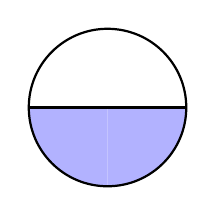
\begin{tikzpicture}
\fill[blue!30] (0,0) -- (0,-1) arc (270:180:1) circle;
\fill[blue!30] (0,0) -- (0,-1) arc (270:360:1) circle;

 \draw[thick] (0,0) circle [radius=1];
 
 \foreach \angle in {0,180}
 	\draw[thick] (0,0) -- (\angle:1);
\end{tikzpicture}
\quad
(b)
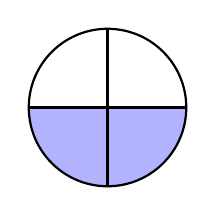
\begin{tikzpicture}
 \fill[blue!30] (0,0) -- (0,-1) arc (270:180:1) circle;
\fill[blue!30] (0,0) -- (0,-1) arc (270:360:1) circle;

 \draw[thick] (0,0) circle [radius=1];
 
\foreach \angle in {0,90,180,270}
 	\draw[thick] (0,0) -- (\angle:1);
\end{tikzpicture}
\quad
(c)
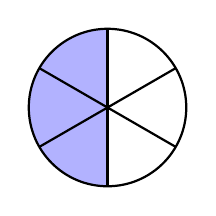
\begin{tikzpicture}
 \fill[blue!30] (0,0) -- (0,1) arc (90:270:1) circle;

 \draw[thick] (0,0) circle [radius=1];
 
\foreach \angle in {30,90,150,210,270,330}
 	\draw[thick] (0,0) -- (\angle:1);
\end{tikzpicture}
\quad
(d)
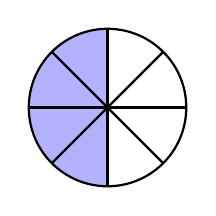
\begin{tikzpicture}
 \fill[blue!30] (0,0) -- (0,1) arc (90:270:1) circle;

 \draw[thick] (0,0) circle [radius=1];
 
\foreach \angle in {0,45,90,135,180,225,270,315}
 	\draw[thick] (0,0) -- (\angle:1);
\end{tikzpicture}

\item Reduce the following fractions to simplest form:\\

a) $\frac{48}{60}$ \quad (b) $\frac{150}{60}$ \quad (c) $\frac{84}{98}$ \quad (d) $\frac{12}{52}$ \quad (e) $\frac{7}{28}$

\item Compare the fractions and put an appropriate sign.\\

(a) $\frac{3}{6} \ \square \ \frac{5}{6} \quad$ (b) $\frac{1}{7} \ \square \ \frac{1}{4} \quad$ (c) $\frac{4}{5} \ \square \ \frac{5}{5} \quad$ (d) $\frac{3}{5} \ \square \ \frac{2}{3} \quad$ 
(e) $\frac{3}{4} \ \square \ \frac{2}{8} \quad$ (f) $\frac{3}{7} \ \square \ \frac{4}{9}$

\item Ila read 25 pages of a book containing 100 pages. Lalita read 25 of the same book. Who read less?

\item In a class A of 25 students, 20 passed in first class; in another class B of 30
students, 24 passed in first class. In which class was a greater fraction of students
getting first class?

\item Fill in the missing fractions.\\

(a) $\frac{7}{10} - \ \square = \frac{3}{10} \quad$ (b) $\square - \frac{3}{21} = \frac{5}{21} \quad$ (c) $\square - \frac{3}{5} = \frac{3}{5} \quad$ (d) $\square + \frac{5}{27} = \frac{12}{27} \quad$ 

\item 
\begin{enumerate}
\item Javed was given $\frac{5}{7}$ of a basket of oranges. What fraction of oranges was left in the basket?

\item Solve\\
(i) $\frac{2}{3} + \frac{1}{7} \quad$ (ii) $\frac{3}{10} + \frac{7}{15} \quad$ (iii) $\frac{4}{9} + \frac{2}{7} \quad$ (iv) $\frac{2}{3} + \frac{3}{4} + \frac{1}{2} \quad$ (v) $4\frac{2}{3} + 3\frac{1}{4} \quad$
(vi) $\frac{1}{2} + \frac{1}{3} + \frac{1}{6}$
\end{enumerate}
\end{enumerate}


%\vspace*{0.2cm}
%\begin{center}
%{\bf ************************************}
%\end{center}

\end{document}